\subsection{Technical Overview of GCP [Shoaib Bin Anwar]}
%
Google Cloud Platform is one of the most used public cloud platforms and is still continuing to grow. It offers a cloud services that run on same infrastructure that Google hosts their product such as Google search, Gmail and Youtube. After Launching of Google App Engine, we have seen other services introduced and the list is continuing to rise.
%
% \subsection{CI-CD Process}
%
% How to setup CI-CD on the tool?


\subsubsection{Setting up a CI/CD pipeline for data-processing workflow}
%
Setting up a continuous integration/continuous deployment is done by implementing CI/CD methods with manage products on Google cloud. The methods are version control (git), build, test and deploy of application, and isolate production environment from  development and staging environment.
%
\subsubsection{Deployment Architecture}
%
\begin{itemize}
    \item  \textbf{Cloud Build} is a service to create CI/CD pipelines for building, deploying, and testing.  It is a series of steps and each step is run in Docker Container. 
    \item \textbf{Cloud Composer} is used for users to manage entire Google Cloud Platform (GCP) pipeline which includes create, schedule, monitor, and manage complex workflows.
    \item \textbf{Dataflow} is the server-less execution service from GCP for data-processing pipelines written using Apache Beam. Apache Beam is an open-source, unified model for defining both batch and streaming data-parallel processing pipelines.
\end{itemize}

\subsubsection{The CI/CD pipeline of GCP}
%
 Cloud Build packages the sample application into a JAR file using the Maven Builder or Gradle Builder. Both are container with Maven or Gradle  installed in it. They run the task when a build step is configured. Cloud Build uploads the JAR file to cloud storage, runs unit tests on data-processing workflow code and deploys the workflow code to the Cloud Composer. Then Cloud Composer picks up the JAR file and runs the data-processing job on Data-flow. 


% 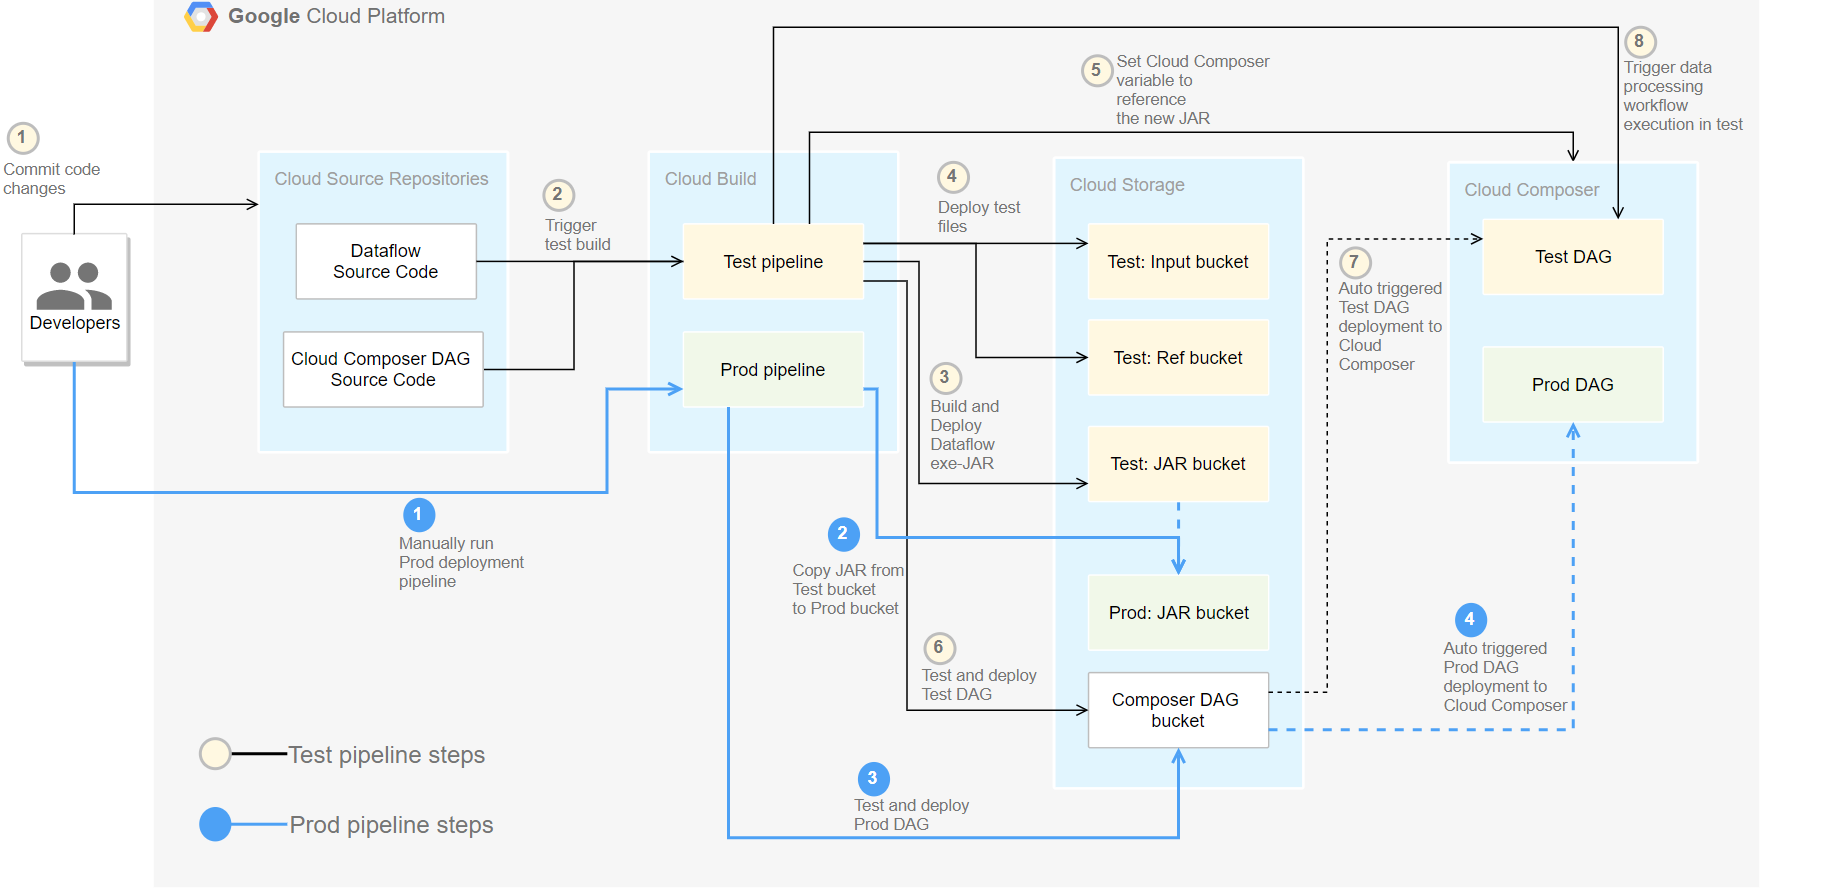
\includegraphics[scale=0.55]{images/shoaib/cicd-pipeline-for-data-processing-1-diagram-pipeline.png}

\begin{figure}[h]
    \centering
    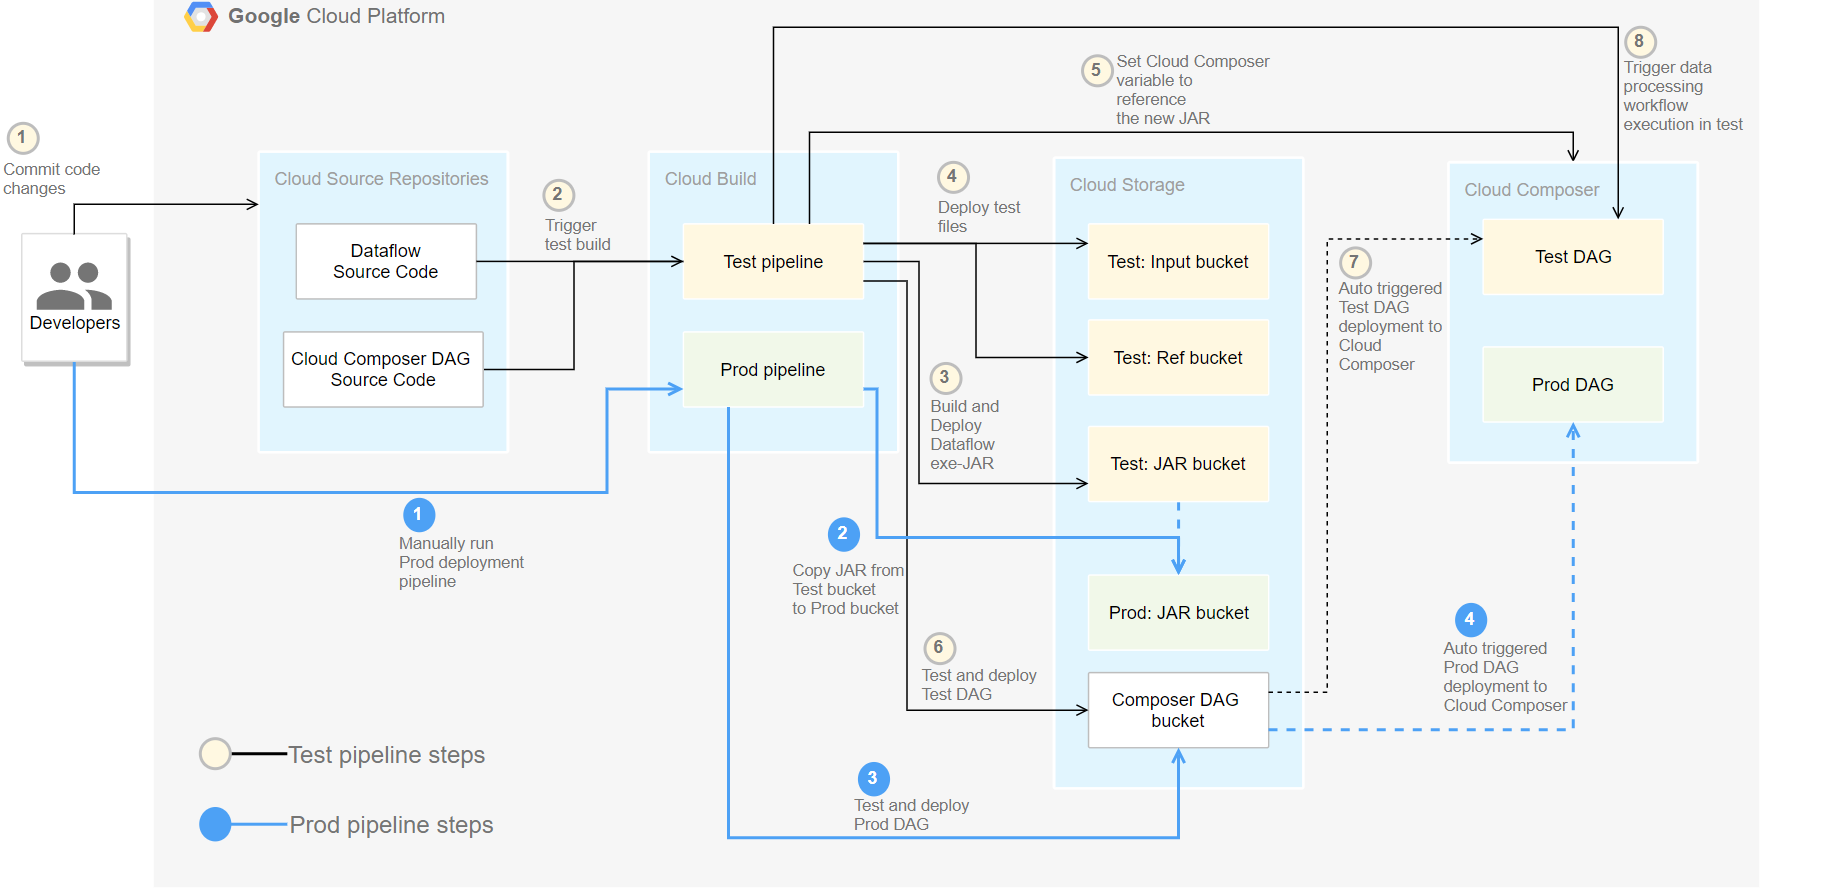
\includegraphics[scale=0.53]{images/shoaib/cicd-pipeline-for-data-processing-1-diagram-pipeline.png}
    \caption{Workflow of CI/CD pipeline in GCP.} 
    \label{fig:gcp_cicd}
\end{figure}
%
We can see in the figure~\ref{fig:gcp_cicd},  the deployments to the test and production environments are separated into two different cloud Build pipelines- a test and a production pipeline.\footnote{https://cloud.google.com/architecture/cicd-pipeline-for-data-processing\#the\_cicd\_pipeline} 
\newline In test pipeline, from the figure we can see that if developer commits something in the code repository, it triggers a test build in Cloud Build. Then Cloud Build builds JAR file and deploys it to the test JAR bucket on Cloud Storage. At the same time, Cloud Build deploys the test files to the test-input bucket and test reference bucket on cloud storage. Cloud Build also sets the variable to reference new JAR file. It also tests DAG and deploys it to the Composer DAG bucket and then DAG file is deployed to Cloud Composer Test DAG. Finally, Cloud Build triggers data processing workflow execution in test. 

On the other hand, in the production pipeline, developers run production deployment pipeline manually. Cloud Build copies the JAR from Test bucket to Production bucket and tests the DAG and deploy the DAG to the Composer DAG bucket. Then, the DAG file is deployed to Cloud Composer. 


%
%
\subsubsection{Pricing}
%
Google Cloud Platform has no up-front costs, pay-as-you-go services, and no fees for termination. In addition, GCP stands out for for its discounts. 
%
\subsubsection{Advantages}
%
GCP probably benefits from the simple fact that Google owns it. Apart from that, there are some benefits of using GCP. Google Cloud Platform(GCP) is designed for cloud-native businesses and is committed to open source and portability. The other significant advantage is price advantages over the other cloud providers, along with frequent discount offers. 


%
\subsubsection{Disadvantages}
%
GCP has disadvantages like other cloud platform. One of the disadvantages is that GCP is still growing. It has fewer features if we compare it with AWS and Azure. Another disadvantage is about the documentation of GCP as it lacks visual description along with textual descriptions\cite{inproceedingss}. We know that visual description like diagram helps the developer to understand the flow of work. So, it is very difficult for the readers to understand the documentation without enough graphs and diagrams.
%
